\documentclass[11pt, xcolor={dvipsnames}, usepdftitle=false]{beamer}
\usepackage{presentation}
\usepackage[brazil]{babel}
\usepackage[utf8]{inputenc}
\usepackage{graphicx}
\hypersetup{pdfpagemode=UseNone, hidelinks, pdfdisplaydoctitle=true,%
pdftitle={Reserva de Salas -- Apresentação de Banca}}

\input{../../../out/drive-links.tex}

\title{Reserva de Salas}
\author{José Ronaldo dos Santos Júnior\\[2mm]{\small Orientador: Prof.\ Gustavo Queiroz Silveira}}
\date{Ciência da Computação -- Centro Universitário Filadélfia\\[1mm]Londrina, Junho de 2026}

\begin{document}
\frame{\titlepage}

% ---- Objetivos e Motivações ----
\begin{frame}
\frametitle{Objetivos e Motivações}
\textbf{Problema:}
\begin{itemize}
\item Gerenciamento de salas dependia de planilhas e controle manual
\item Trocas de horário, alta demanda e restrições tornavam o processo complexo
\item Risco de conflitos de agendamento, retrabalho e perda de rastreabilidade
\end{itemize}
\vspace{3mm}
\textbf{Objetivo principal:} desenvolver uma solução de agendamento de salas para a UniFil.
\begin{itemize}
\item Centralizar as informações de agendamento
\item Automatizar o fluxo de solicitação e aprovação de reservas
\item Manter histórico de alterações
\end{itemize}
\end{frame}

% ---- Tecnologias ----
\begin{frame}
\frametitle{Tecnologias Utilizadas}
\begin{itemize}
\item \textbf{Linguagens de Programação:}
\begin{itemize}
\item \textit{Back-end}: Java --- consolidado no mercado corporativo
\item \textit{Front-end}: JavaScript --- padrão para interfaces web
\end{itemize}
\item \textbf{Banco de Dados:} PostgreSQL --- maturidade e compatibilidade com os frameworks adotados
\item \textbf{Frameworks de Desenvolvimento:}
\begin{itemize}
\item \textit{Front-end}: React --- interfaces reativas e componentizadas
\item \textit{Back-end}: Spring Boot --- exposição de APIs REST sobre o ecossistema Spring
\end{itemize}
\end{itemize}
\end{frame}

% ---- Separador: Diagramas ----
\begin{frame}
\heading{Diagramas}
\end{frame}

% ---- Workflow AS-IS ----
\begin{frame}
\frametitle{Workflow AS-IS (BPMN)}
\begin{figure}
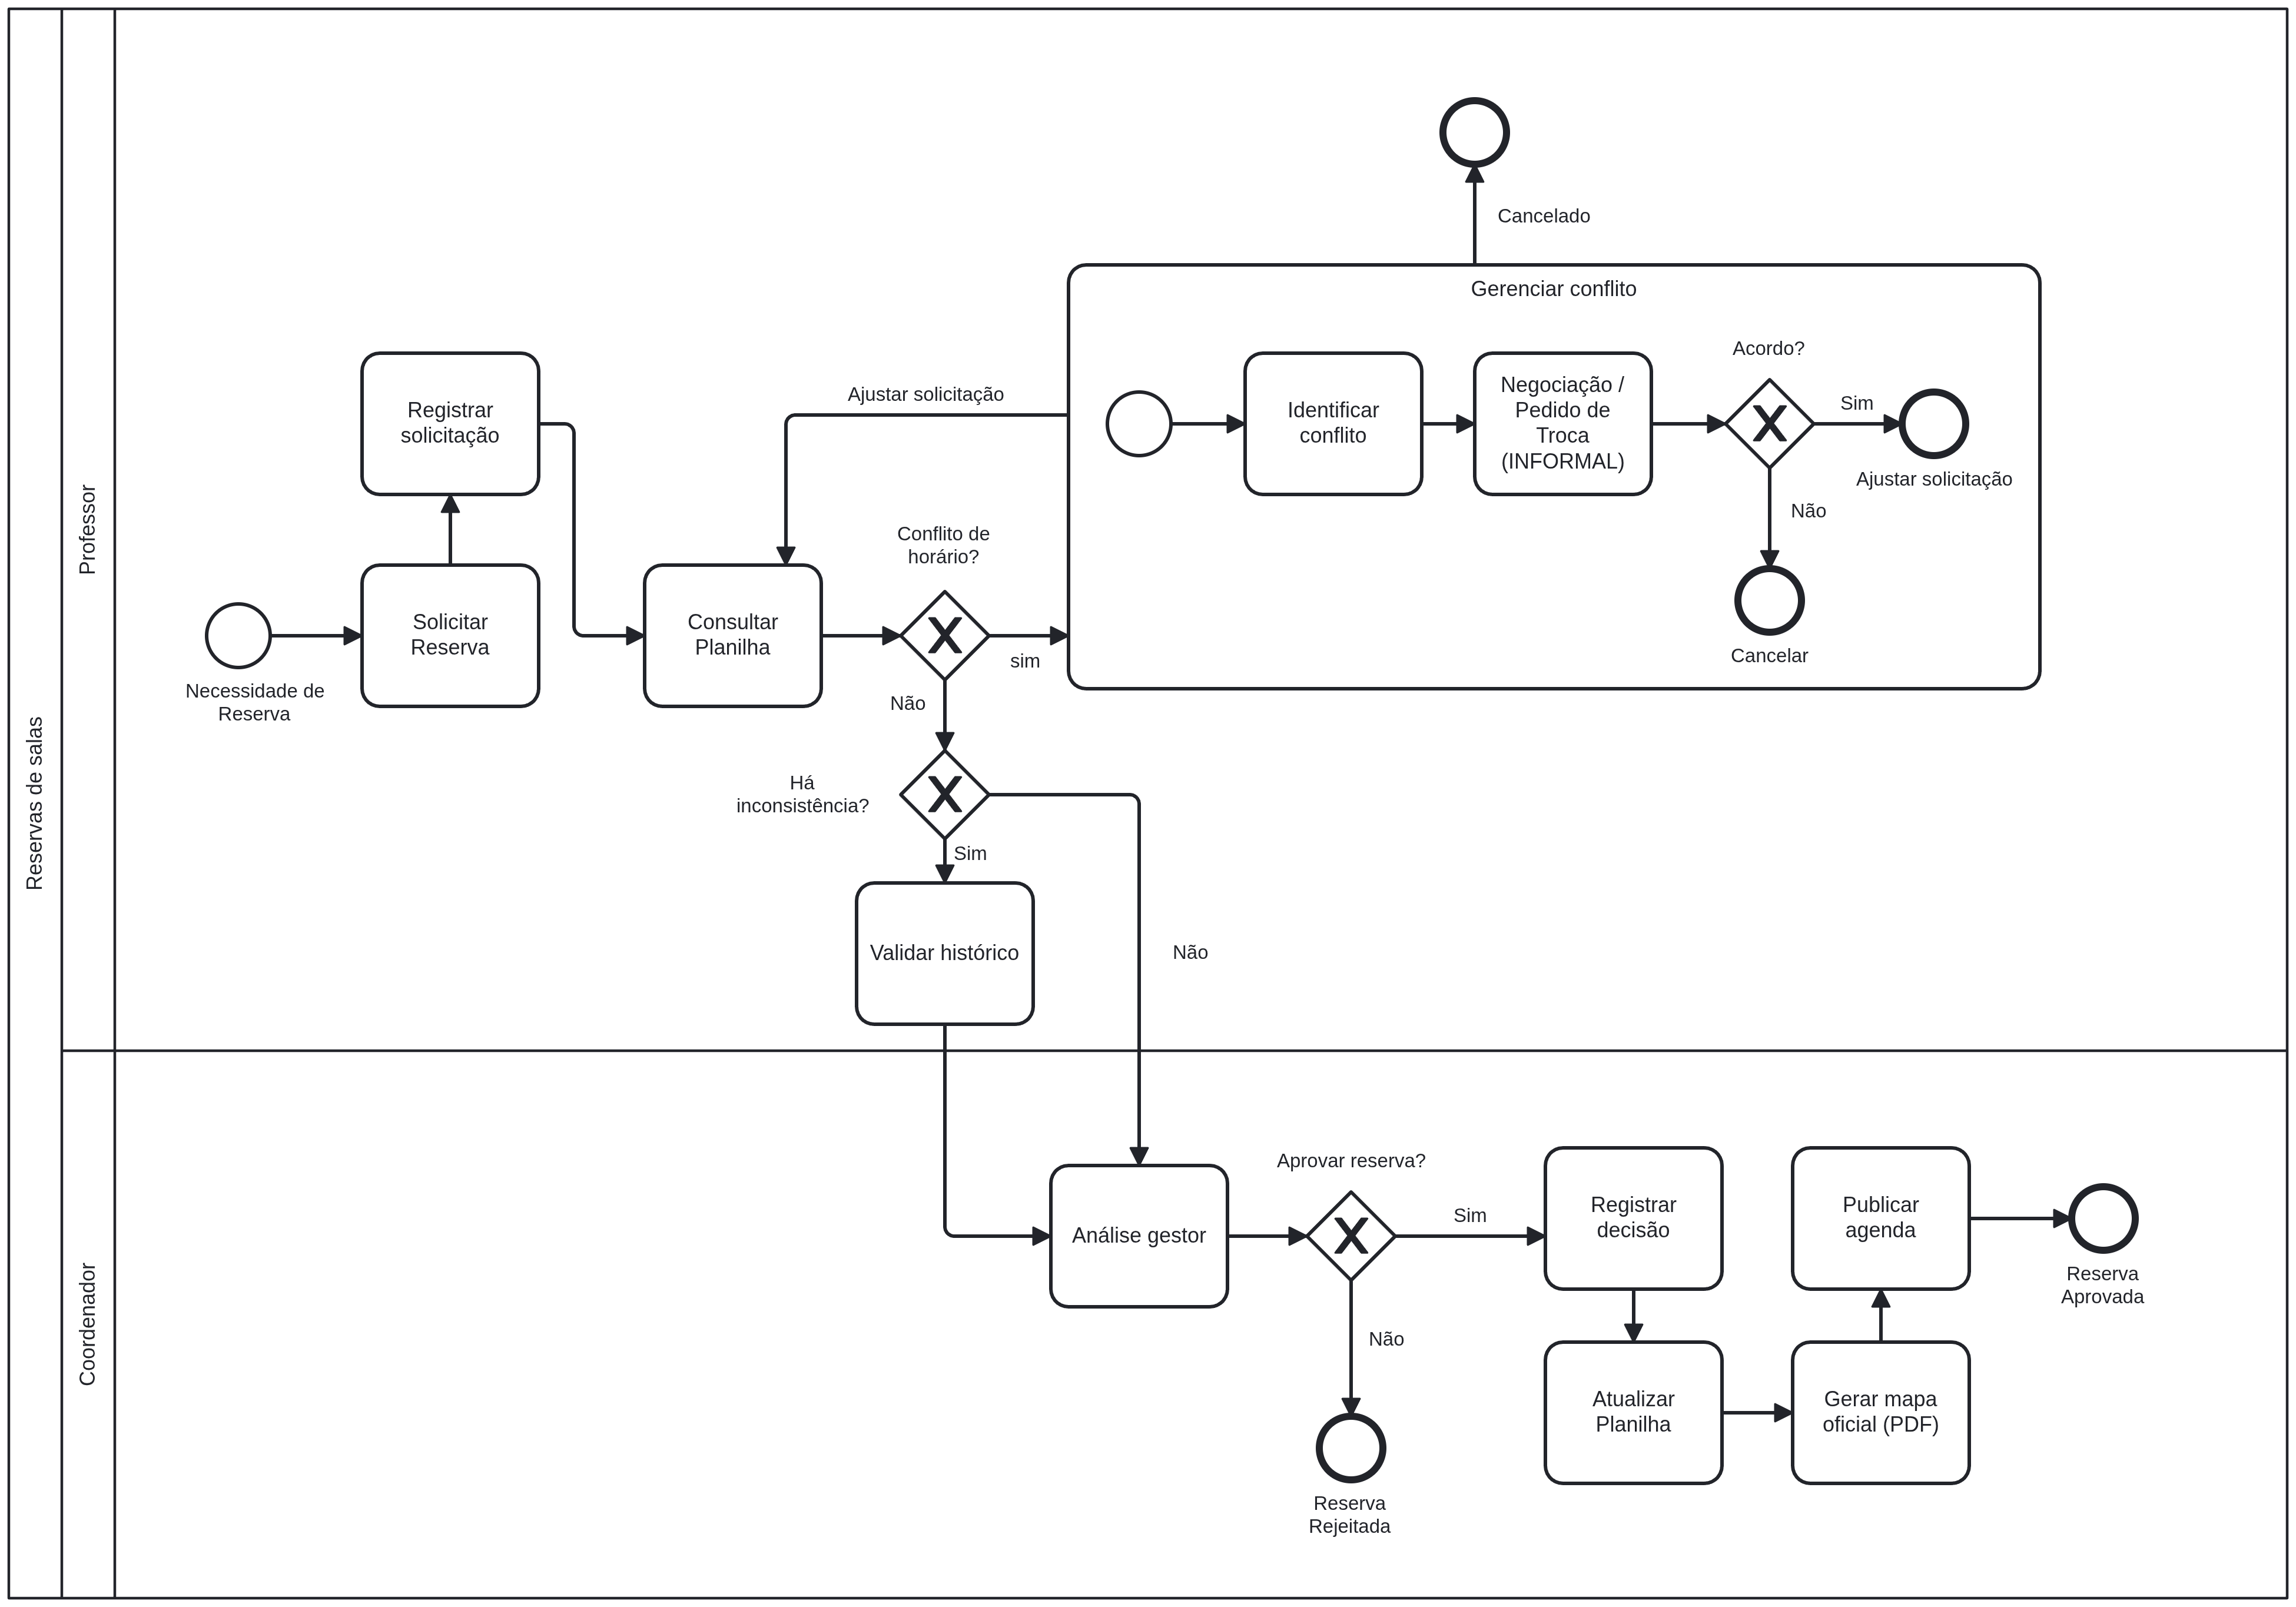
\includegraphics[width=\textwidth,height=0.72\textheight,keepaspectratio]{../relatorio-estagio/imagens/workflow-as-is.png}
\caption{Fluxo manual via planilha: consulta, negociação informal de conflitos e atualização/publicação manuais geram risco de erro e retrabalho}
\end{figure}
\end{frame}

% ---- Diagrama de Caso de Uso ----
\begin{frame}
\frametitle{Diagrama de Caso de Uso}
\begin{figure}
\includegraphics[width=\textwidth,height=0.7\textheight,keepaspectratio]{../../../out/src/plantuml/usecasediagram.png}
\end{figure}
\end{frame}

% ---- Atores ----
\begin{frame}
\frametitle{Atores do Sistema}
\begin{itemize}
\item \textbf{sa\_professor} --- usuário comum:
\begin{itemize}
\item Autenticação, gerenciamento de salas e agendamentos
\item Geração de relatórios e consulta ao histórico
\end{itemize}
\item \textbf{sa\_coordenador} --- especialização de \textbf{sa\_professor}:
\begin{itemize}
\item Todas as permissões de professor
\item Acesso ao gerenciamento de usuários
\end{itemize}
\end{itemize}
\end{frame}

% ---- DER ----
\begin{frame}
\frametitle{Modelagem do Banco de Dados (DER)}
\begin{figure}
\includegraphics[width=\textwidth,height=0.7\textheight,keepaspectratio]{../../../out/src/plantuml/der-horizontal.png}
\end{figure}
\end{frame}

% ---- Diagrama de Componentes ----
\begin{frame}
\frametitle{Diagrama de Componentes --- Visão Geral dos Módulos}
\begin{figure}
\includegraphics[width=\textwidth,height=0.7\textheight,keepaspectratio]{../../../out/src/plantuml/componentes.png}
\end{figure}
\end{frame}

% ---- Diagramas de Classes ----
\begin{frame}
\frametitle{Diagrama de Classe --- Usuário}
\begin{figure}
\includegraphics[width=\textwidth,height=0.7\textheight,keepaspectratio]{../../../out/src/plantuml/classe/user.png}
\end{figure}
\end{frame}

\begin{frame}
\frametitle{Diagrama de Classe --- Sala}
\begin{figure}
\includegraphics[width=\textwidth,height=0.7\textheight,keepaspectratio]{../../../out/src/plantuml/classe/room.png}
\end{figure}
\end{frame}

\begin{frame}
\frametitle{Diagrama de Classe --- Evento}
\begin{figure}
\includegraphics[width=\textwidth,height=0.7\textheight,keepaspectratio]{../../../out/src/plantuml/classe/event.png}
\end{figure}
\end{frame}

\begin{frame}
\frametitle{Diagrama de Classe --- Autenticação}
\begin{figure}
\includegraphics[width=\textwidth,height=0.7\textheight,keepaspectratio]{../../../out/src/plantuml/classe/auth.png}
\end{figure}
\end{frame}

% ---- Diagrama de Estado: Usuário ----
\begin{frame}
\frametitle{Diagrama de Estado --- Usuário}
\begin{figure}
\includegraphics[width=\textwidth,height=0.7\textheight,keepaspectratio]{../../../out/src/plantuml/estado/user_status.png}
\end{figure}
\end{frame}

% ---- Diagramas de Sequência: Usuário e Sala (representativos) ----
\begin{frame}
\frametitle{Diagrama de Sequência --- Criar Usuário}
\begin{figure}
\includegraphics[width=\textwidth,height=0.7\textheight,keepaspectratio]{../../../out/src/plantuml/sequencia/user/create_user.png}
\end{figure}
\end{frame}

\begin{frame}
\frametitle{Diagrama de Sequência --- Criar Sala}
\begin{figure}
\includegraphics[width=\textwidth,height=0.7\textheight,keepaspectratio]{../../../out/src/plantuml/sequencia/room/create_room.png}
\end{figure}
\end{frame}

% ---- Diagrama de Implantação ----
\begin{frame}
\frametitle{Diagrama de Implantação}
\begin{figure}
\includegraphics[width=\textwidth,height=0.7\textheight,keepaspectratio]{../../../out/src/plantuml/deployment.png}
\end{figure}
\end{frame}

% ---- Separador: Telas ----
\begin{frame}
\heading{Apresentação do Sistema}
\end{frame}

% ---- Transição para demonstração ao vivo ----
\begin{frame}
\frametitle{Demonstração}
\begin{itemize}
\item Login e autenticação
\item Cadastro e gerenciamento de salas
\item Busca de salas disponíveis
\item Solicitação e acompanhamento de reservas
\item Grade de horários
\end{itemize}
\vspace{4mm}
\end{frame}

% ---- Artefatos de Requisitos ----
\begin{frame}
\frametitle{Artefatos de Requisitos}
\begin{itemize}
\item \textbf{Documento de Visão}
\item \textbf{Especificação Complementar}
\item \textbf{Glossário}
\item \textbf{Solicitação dos Principais Envolvidos}
\item \textbf{Especificação de Caso de Uso}
\end{itemize}
\end{frame}

% ---- Conceitos de Engenharia de Software Aplicados ----
\begin{frame}
\frametitle{Conceitos de Engenharia de Software Aplicados}
\begin{itemize}
\item \textbf{Clean Architecture (Ports \& Adapters):} camadas Domain, Application e Infrastructure; portas (interfaces) implementadas por adaptadores
\item \textbf{Domain-Driven Design:}
\begin{itemize}
\item Entidades ricas (ex: \texttt{activate()}, \texttt{archive()}, \texttt{restore()})
\item Value Objects (\texttt{UserId}, \texttt{RoomId}, \texttt{BuildingId})
\item Agregados referenciados por ID, mantendo limites de agregado pequenos
\end{itemize}
\item \textbf{Notification Pattern:} validadores que coletam erros (\texttt{validate(Entidade, Notification)}) em vez de lançar exceção por campo
\item \textbf{Monólito Modular:} módulos por domínio (usuário, sala, autenticação) com núcleo compartilhado e comunicação entre módulos via portas
\end{itemize}
\end{frame}

% ---- Conclusão ----
\begin{frame}
\frametitle{Conclusão}
\textbf{Resultados alcançados:}
\begin{itemize}
\item Autenticação e gerenciamento de usuários (professor/coordenador)
\item Cadastro e gerenciamento de salas, recursos e prédios
\item Modelagem completa do sistema (casos de uso, DER, classes, sequência, implantação)
\end{itemize}
\vspace{3mm}
\textbf{Em desenvolvimento:}
\begin{itemize}
\item Fluxo de solicitação e aprovação de reservas
\item Grade de horários e visualização de disponibilidade
\end{itemize}
\end{frame}

% ======================================================================
% Slides de apoio (não apresentados no tempo principal; usar se a banca
% perguntar sobre algum desses diagramas/entidades específicas)
% ======================================================================

\begin{frame}
\heading{Slides de Apoio}
\end{frame}

\begin{frame}
\frametitle{Diagrama de Estado --- Sala}
\begin{figure}
\includegraphics[width=\textwidth,height=0.7\textheight,keepaspectratio]{../../../out/src/plantuml/estado/room_status.png}
\end{figure}
\end{frame}

\begin{frame}
\frametitle{Diagrama de Estado --- Tipo de Sala}
\begin{figure}
\includegraphics[width=\textwidth,height=0.7\textheight,keepaspectratio]{../../../out/src/plantuml/estado/room_type_status.png}
\end{figure}
\end{frame}

\begin{frame}
\frametitle{Diagrama de Estado --- Prédio}
\begin{figure}
\includegraphics[width=\textwidth,height=0.7\textheight,keepaspectratio]{../../../out/src/plantuml/estado/building_status.png}
\end{figure}
\end{frame}

\begin{frame}
\frametitle{Diagrama de Estado --- Recurso}
\begin{figure}
\includegraphics[width=\textwidth,height=0.7\textheight,keepaspectratio]{../../../out/src/plantuml/estado/resource_status.png}
\end{figure}
\end{frame}

\begin{frame}
\frametitle{Diagrama de Sequência --- Buscar Usuário}
\begin{figure}
\includegraphics[width=\textwidth,height=0.7\textheight,keepaspectratio]{../../../out/src/plantuml/sequencia/user/get_user.png}
\end{figure}
\end{frame}

\begin{frame}
\frametitle{Diagrama de Sequência --- Atualizar Usuário}
\begin{figure}
\includegraphics[width=\textwidth,height=0.7\textheight,keepaspectratio]{../../../out/src/plantuml/sequencia/user/update_user.png}
\end{figure}
\end{frame}

\begin{frame}
\frametitle{Diagrama de Sequência --- Atualizar Status do Usuário}
\begin{figure}
\includegraphics[width=\textwidth,height=0.7\textheight,keepaspectratio]{../../../out/src/plantuml/sequencia/user/update_user_status.png}
\end{figure}
\end{frame}

\begin{frame}
\frametitle{Diagrama de Sequência --- Excluir Usuário}
\begin{figure}
\includegraphics[width=\textwidth,height=0.7\textheight,keepaspectratio]{../../../out/src/plantuml/sequencia/user/delete_user.png}
\end{figure}
\end{frame}

\begin{frame}
\frametitle{Diagrama de Sequência --- Buscar Sala}
\begin{figure}
\includegraphics[width=\textwidth,height=0.7\textheight,keepaspectratio]{../../../out/src/plantuml/sequencia/room/get_room_simple.png}
\end{figure}
\end{frame}

\begin{frame}
\frametitle{Diagrama de Sequência --- Atualizar Sala}
\begin{figure}
\includegraphics[width=\textwidth,height=0.7\textheight,keepaspectratio]{../../../out/src/plantuml/sequencia/room/update_room.png}
\end{figure}
\end{frame}

\begin{frame}
\frametitle{Diagrama de Sequência --- Atualizar Status da Sala}
\begin{figure}
\includegraphics[width=\textwidth,height=0.7\textheight,keepaspectratio]{../../../out/src/plantuml/sequencia/room/update_room_status.png}
\end{figure}
\end{frame}

\begin{frame}
\frametitle{Diagrama de Sequência --- Substituir Recursos da Sala}
\begin{figure}
\includegraphics[width=\textwidth,height=0.7\textheight,keepaspectratio]{../../../out/src/plantuml/sequencia/room/replace_room_resources.png}
\end{figure}
\end{frame}

\begin{frame}
\frametitle{Diagrama de Sequência --- Excluir Sala}
\begin{figure}
\includegraphics[width=\textwidth,height=0.7\textheight,keepaspectratio]{../../../out/src/plantuml/sequencia/room/delete_room.png}
\end{figure}
\end{frame}

% ---- Plano B: telas do sistema (caso a demo ao vivo falhe) ----
\begin{frame}
\frametitle{Tela de Login}
\begin{figure}
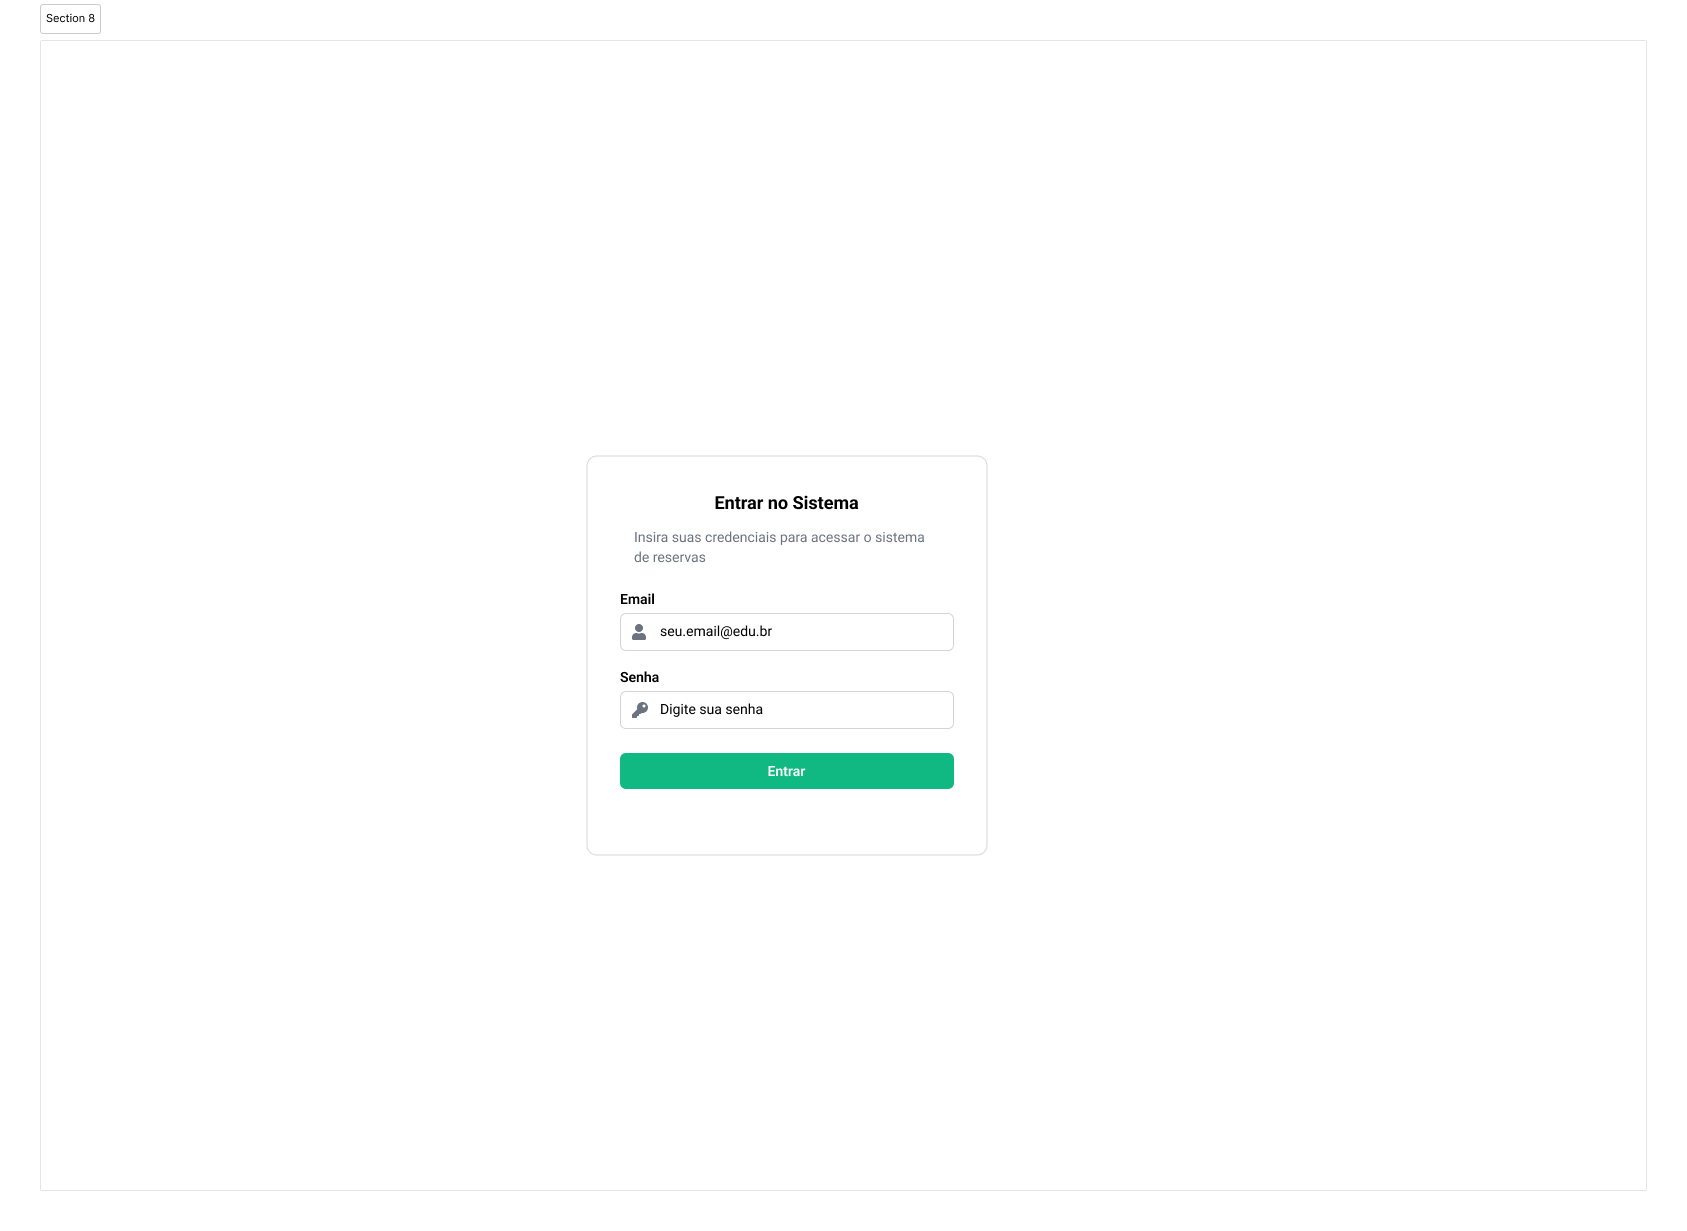
\includegraphics[width=\textwidth,height=0.72\textheight,keepaspectratio]{../relatorio-estagio/imagens/telas/login.png}
\caption{Autenticação com e-mail e senha}
\end{figure}
\end{frame}

\begin{frame}
\frametitle{Gerenciamento de Salas}
\begin{figure}
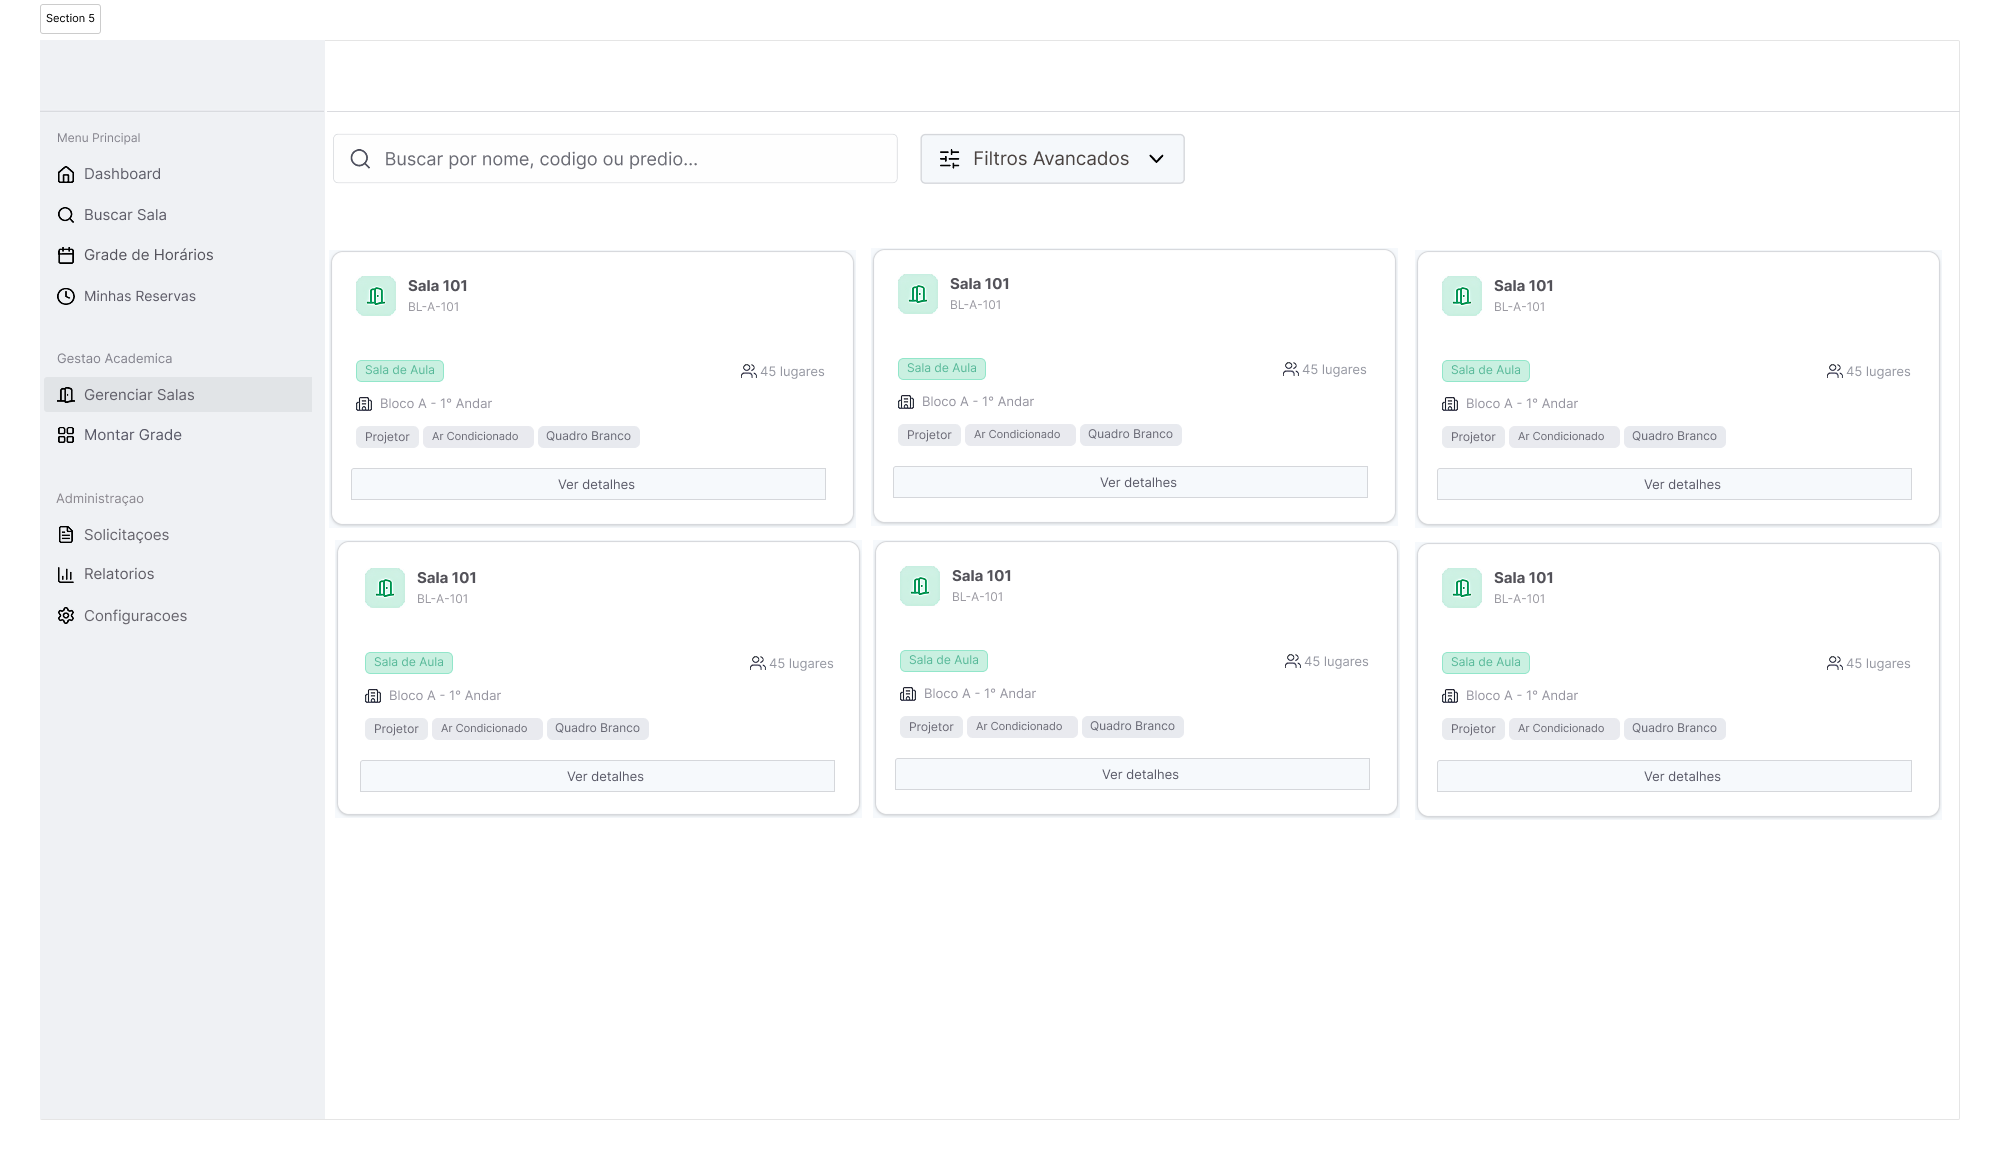
\includegraphics[width=\textwidth,height=0.72\textheight,keepaspectratio]{../relatorio-estagio/imagens/telas/gerenciar-salas.png}
\caption{Visualização, cadastro, edição e remoção de salas}
\end{figure}
\end{frame}

\begin{frame}
\frametitle{Buscar Sala}
\begin{figure}
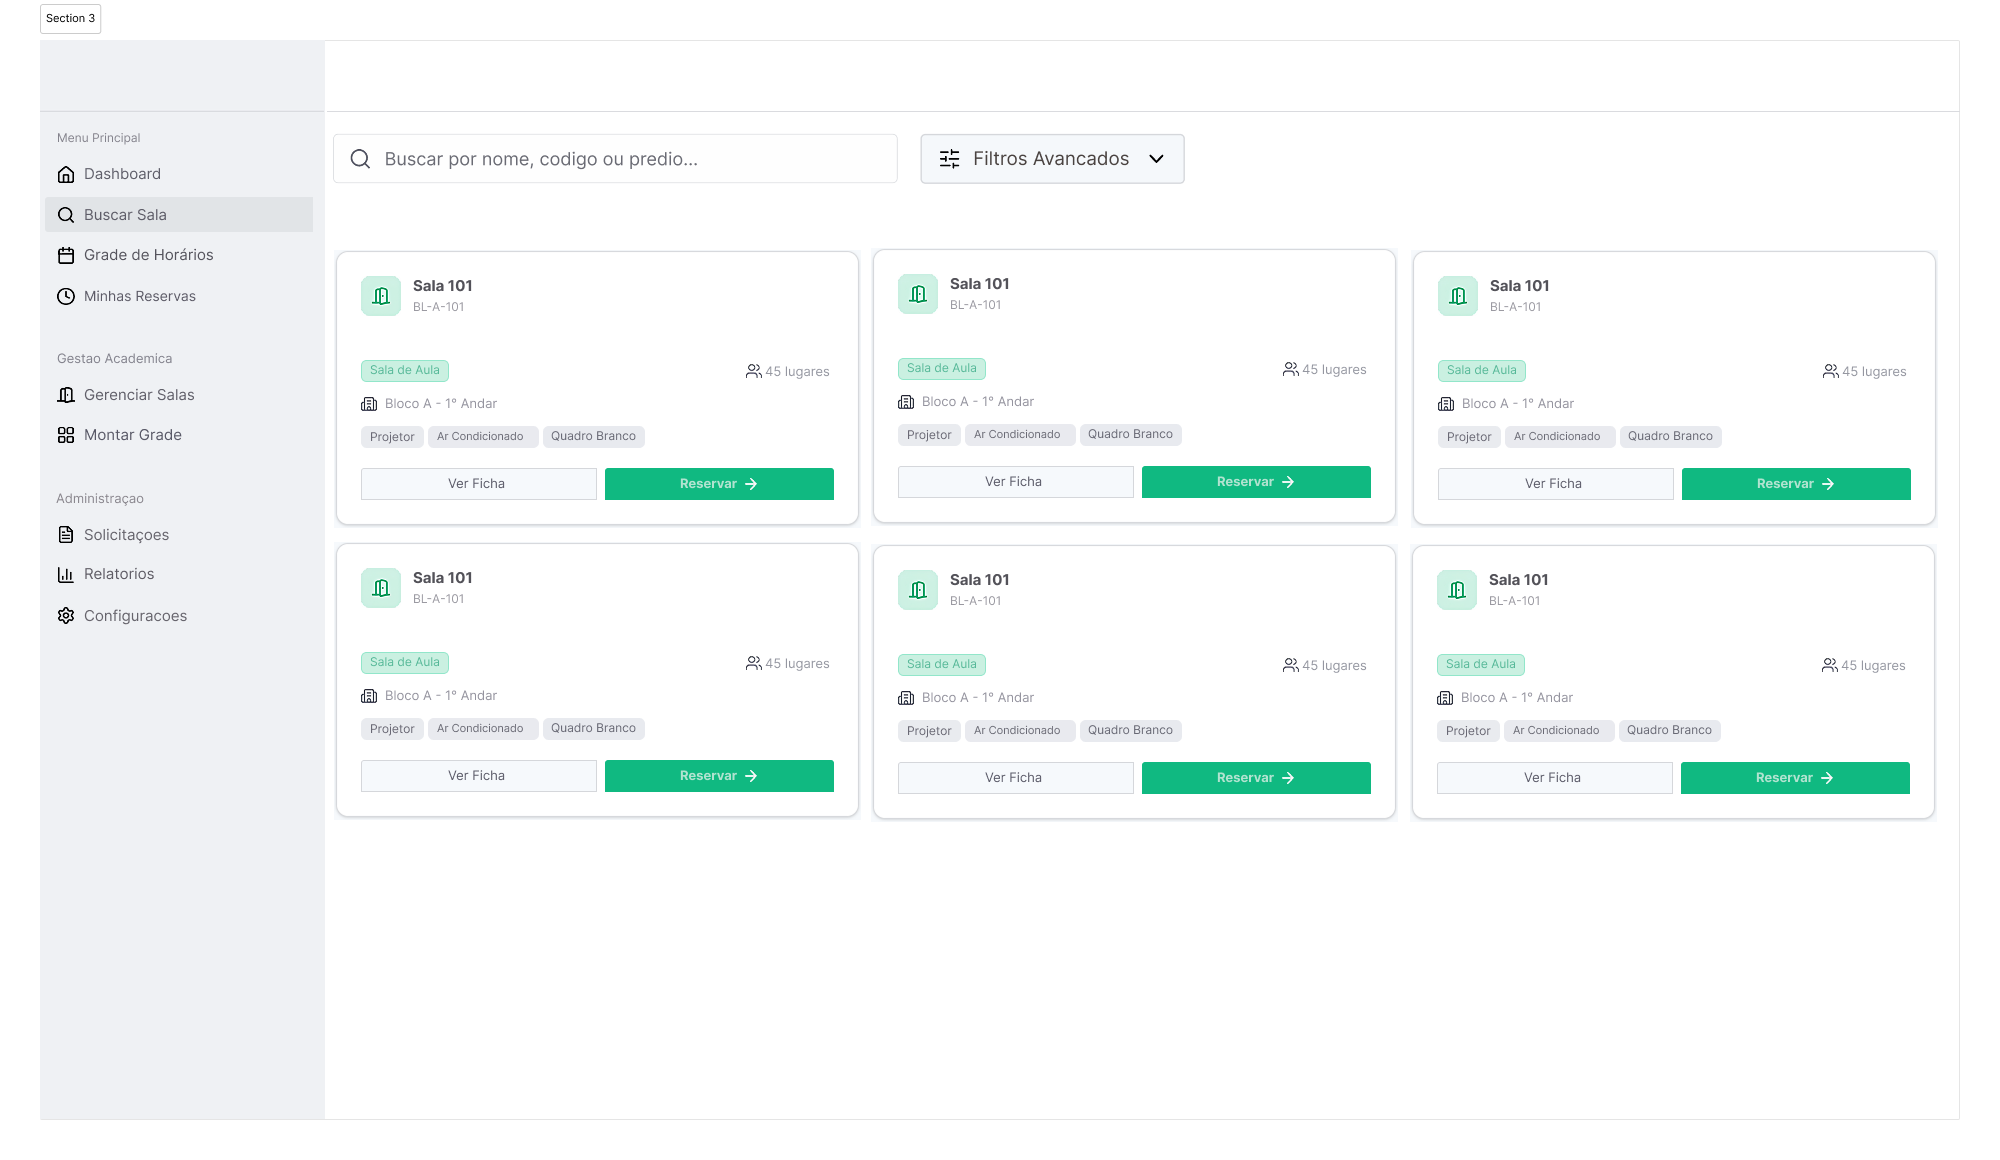
\includegraphics[width=\textwidth,height=0.72\textheight,keepaspectratio]{../relatorio-estagio/imagens/telas/buscar-sala.png}
\caption{Consulta de salas disponíveis}
\end{figure}
\end{frame}

\begin{frame}
\frametitle{Minhas Reservas}
\begin{figure}
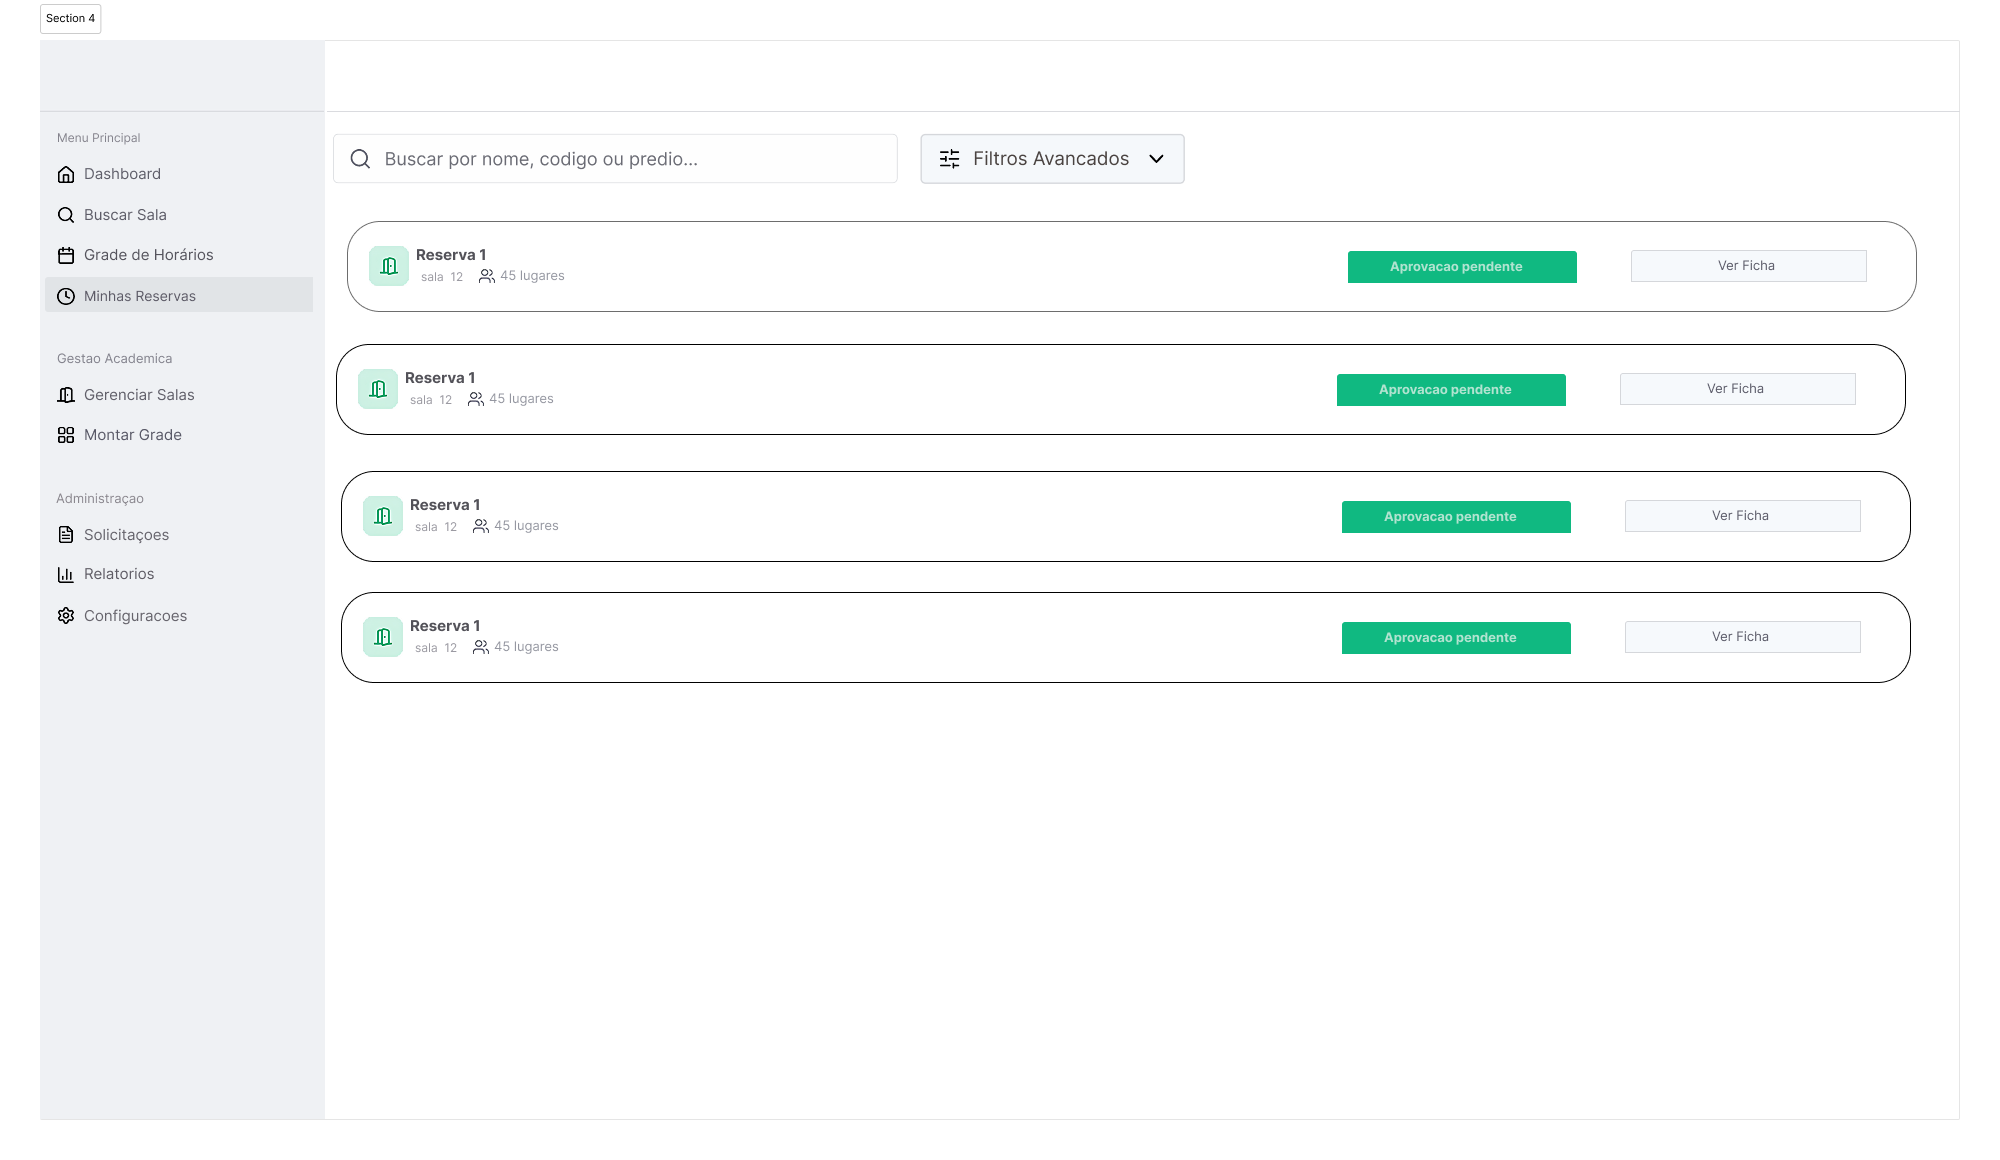
\includegraphics[width=\textwidth,height=0.72\textheight,keepaspectratio]{../relatorio-estagio/imagens/telas/minhas-reservas.png}
\caption{Acompanhamento dos agendamentos realizados}
\end{figure}
\end{frame}

\begin{frame}
\frametitle{Solicitações}
\begin{figure}
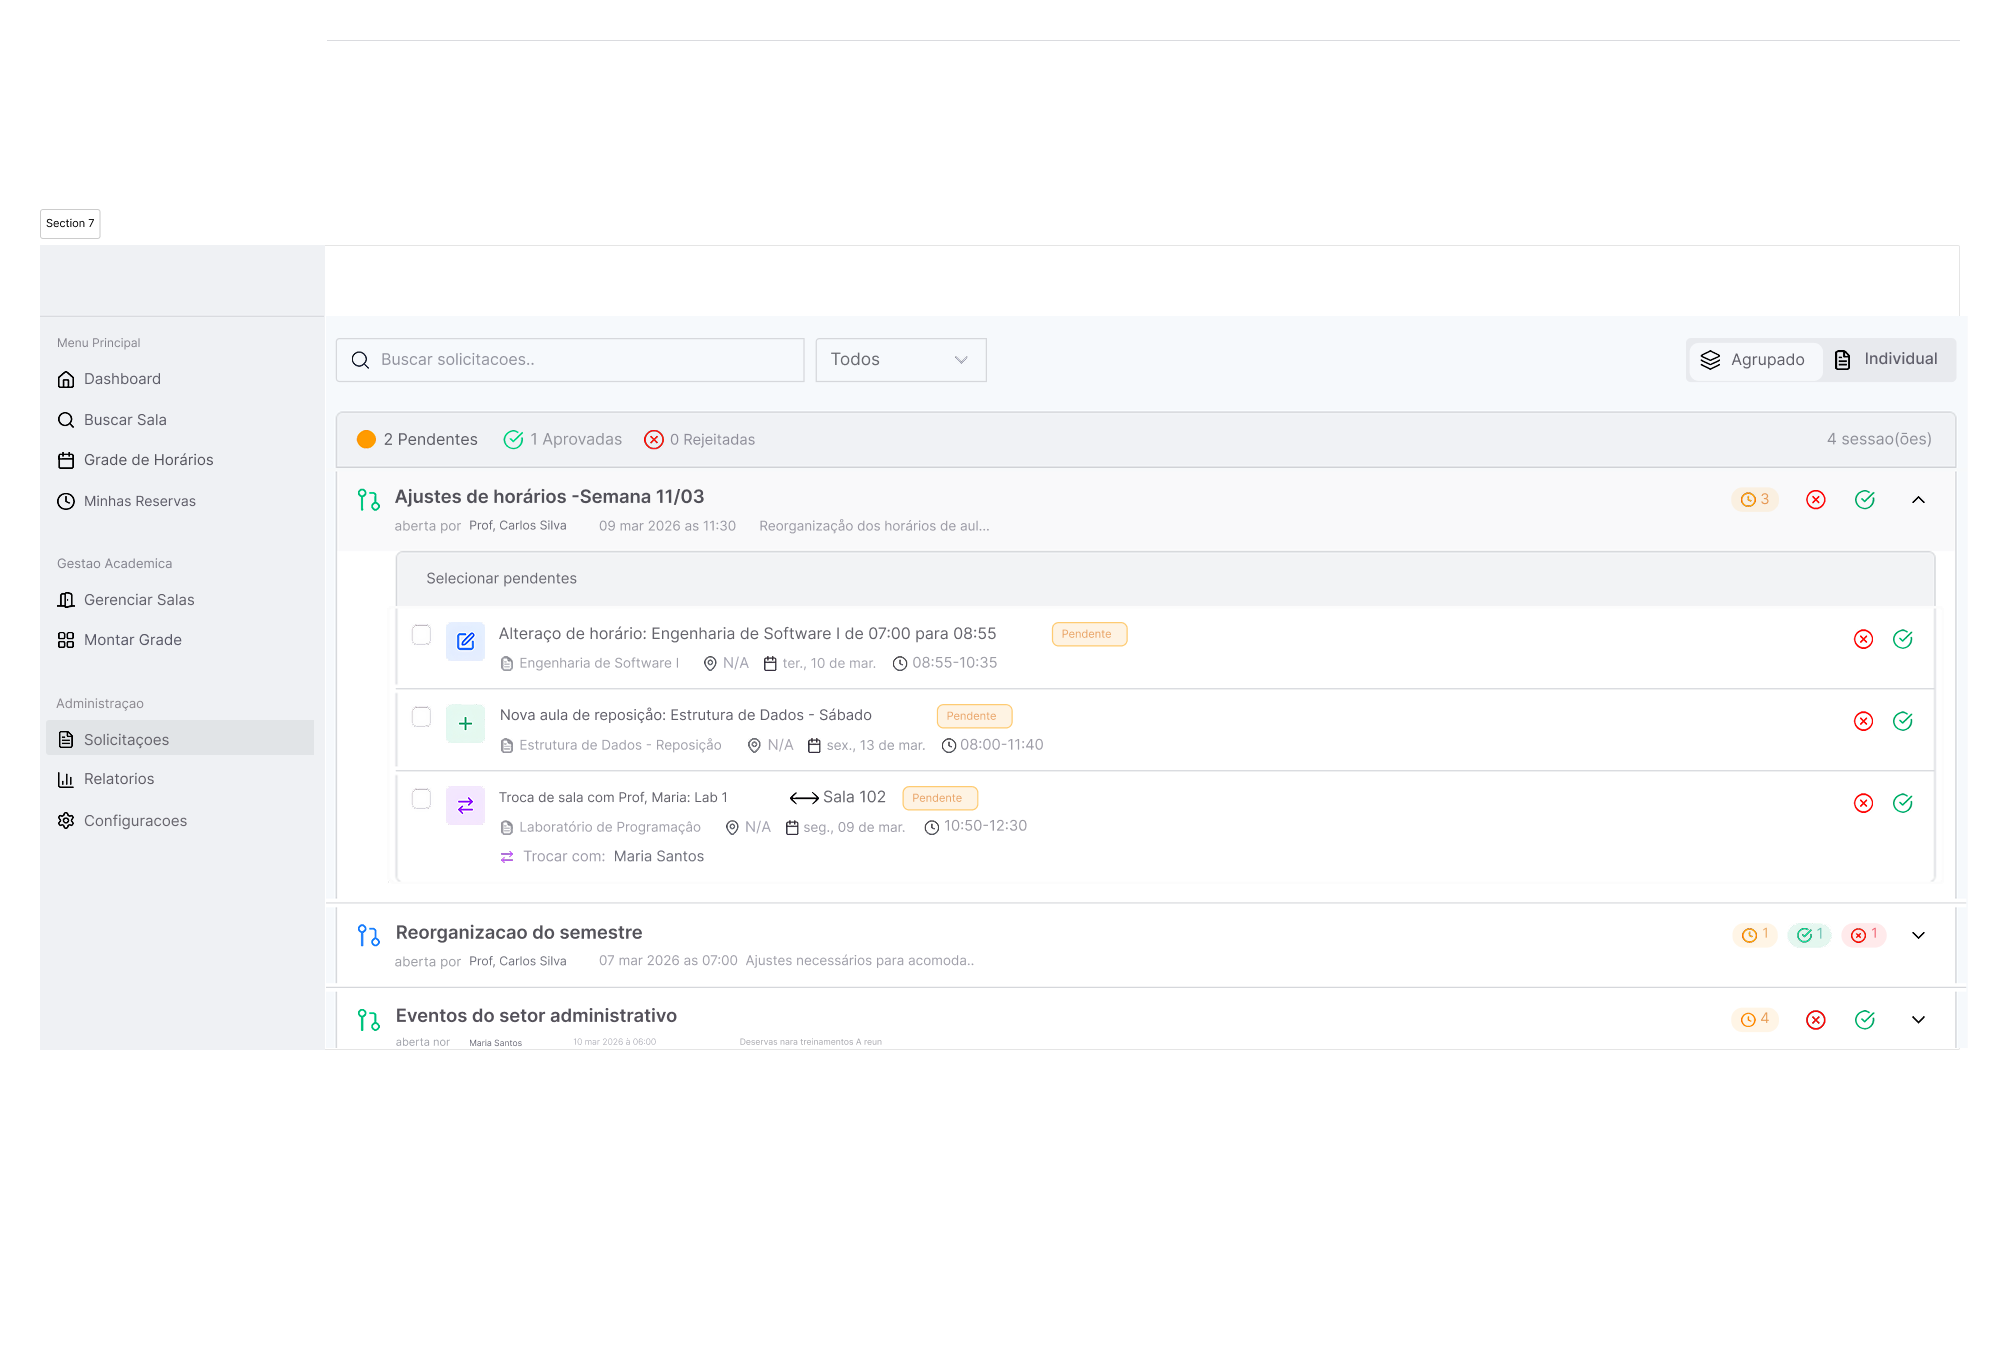
\includegraphics[width=\textwidth,height=0.72\textheight,keepaspectratio]{../relatorio-estagio/imagens/telas/solicitacoes.png}
\caption{Pedidos e seus respectivos status}
\end{figure}
\end{frame}

\begin{frame}
\frametitle{Grade de Horários}
\begin{figure}
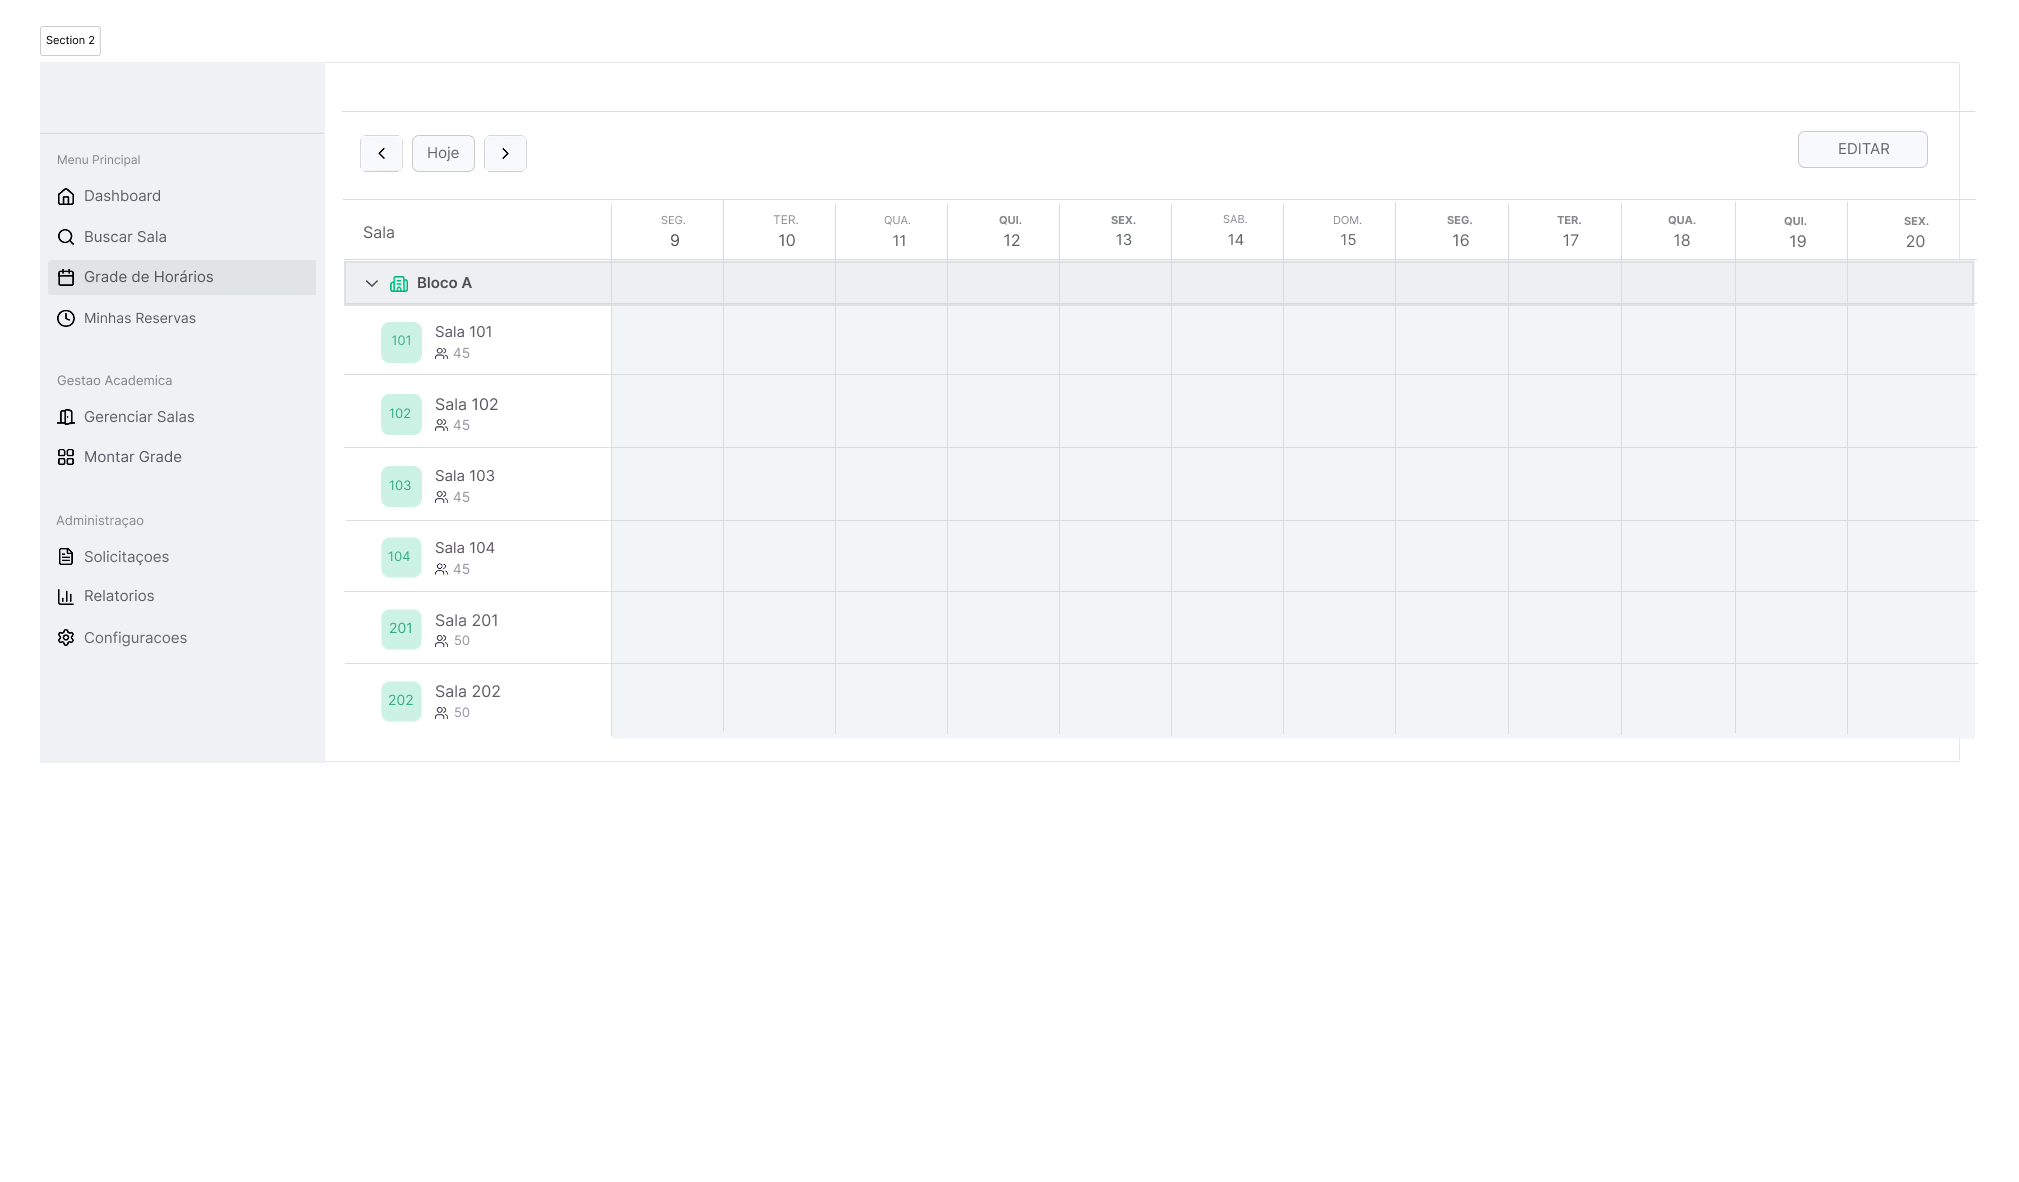
\includegraphics[width=\textwidth,height=0.72\textheight,keepaspectratio]{../relatorio-estagio/imagens/telas/grade-horarios.png}
\caption{Visualização da ocupação e disponibilidade das salas}
\end{figure}
\end{frame}

\begin{frame}
\frametitle{Montar Grade}
\begin{figure}
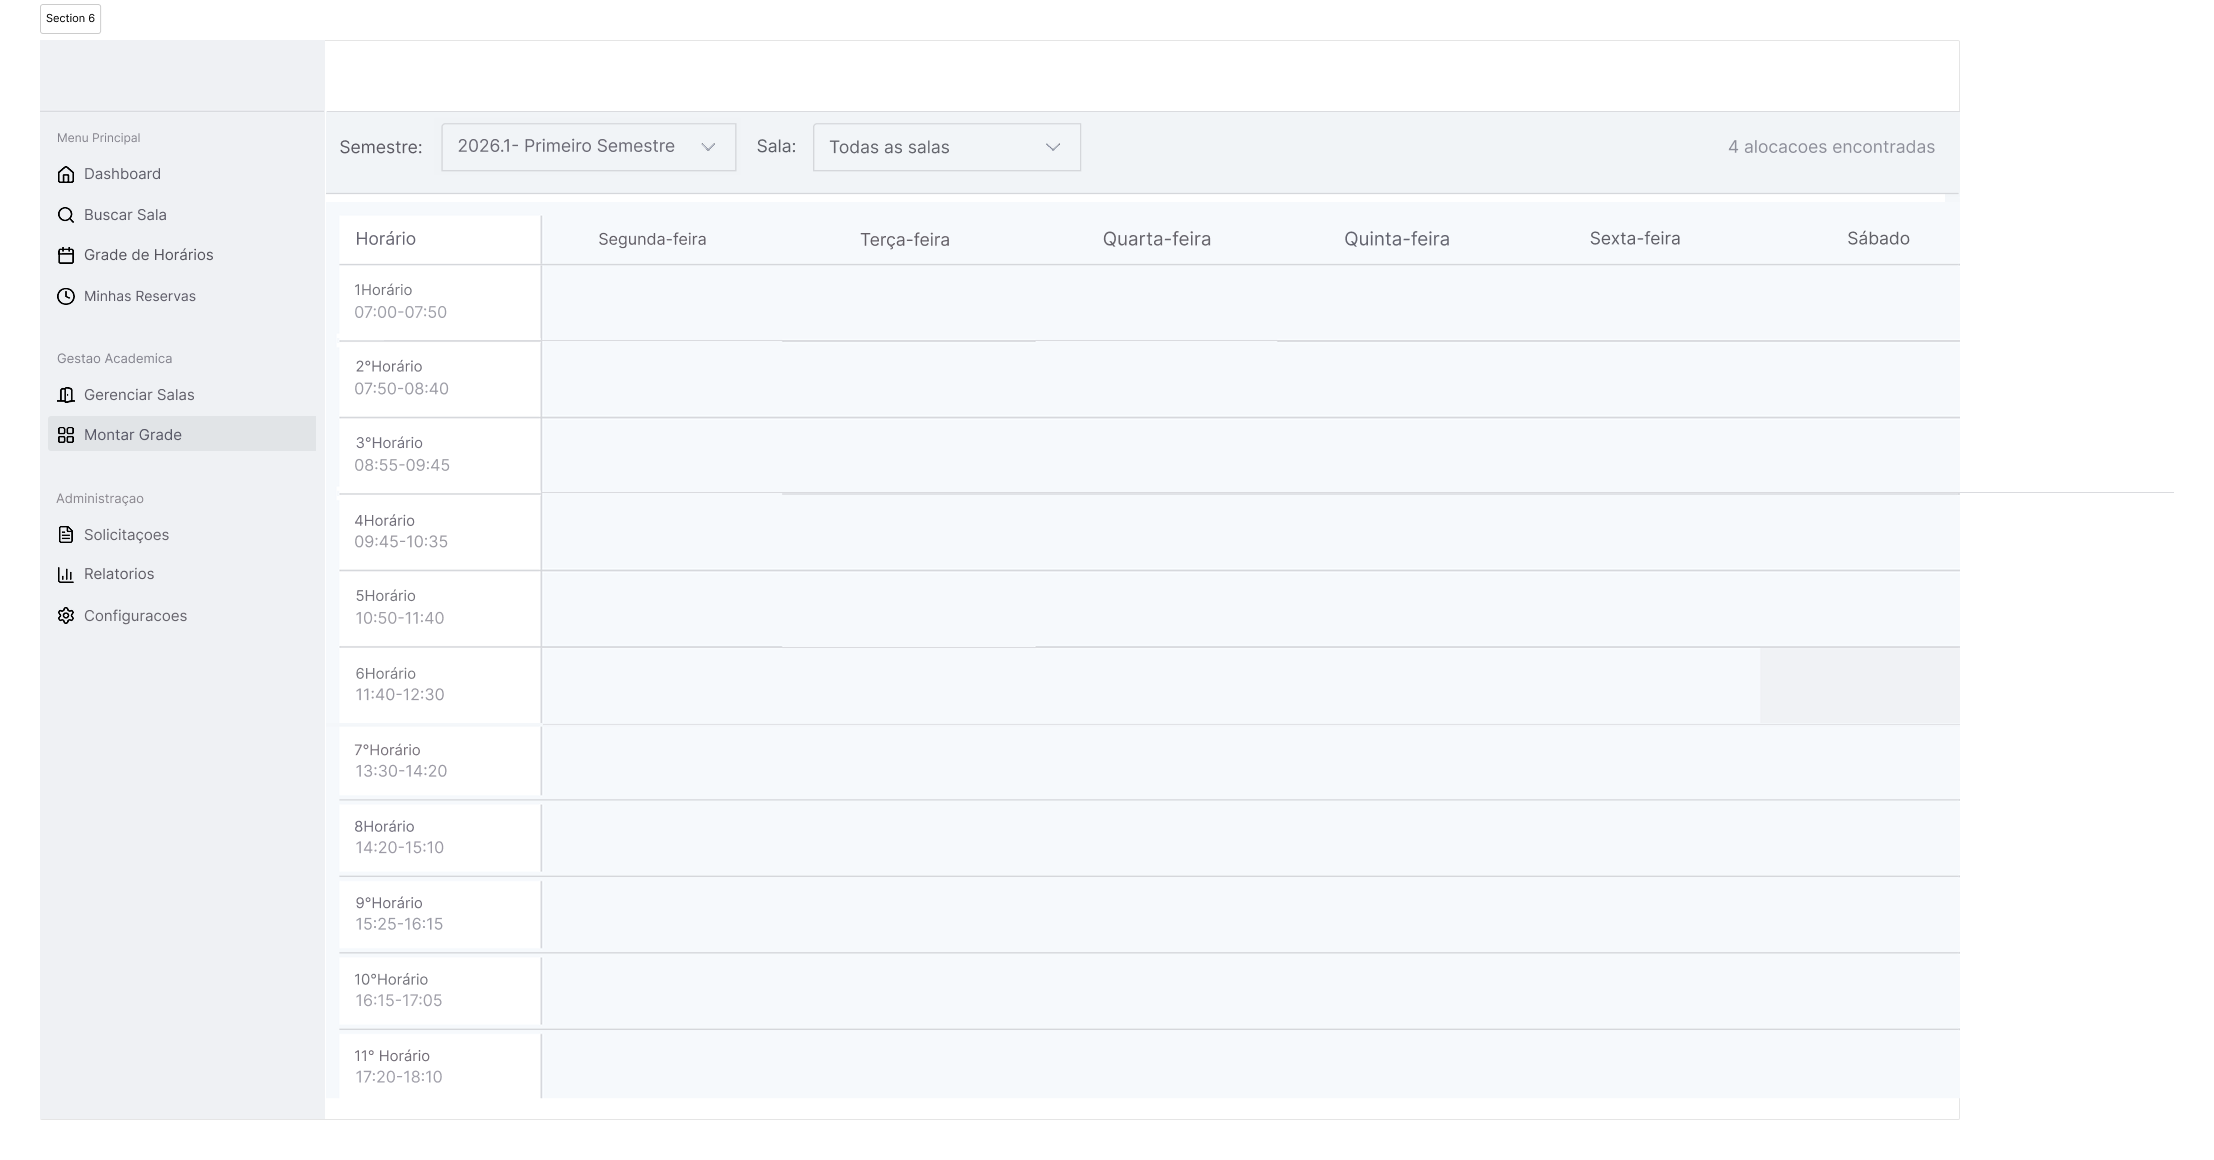
\includegraphics[width=\textwidth,height=0.72\textheight,keepaspectratio]{../relatorio-estagio/imagens/telas/montar-grade.png}
\caption{Estruturação da grade de horários por sala}
\end{figure}
\end{frame}

\lastslide

\end{document}
